\documentclass[12pt, a4paper]{article}


\usepackage{tabularx}
\usepackage{graphicx}
\usepackage[moderate]{savetrees}
\usepackage{hyperref}
\usepackage{float}
\usepackage{rotating}
\hypersetup{
	colorlinks,
	citecolor=black,
	filecolor=black,
	linkcolor=black,
	urlcolor=black
}
\usepackage{bookmark}
\bookmarksetup{numbered}
\usepackage{microtype}


\usepackage{ragged2e}
\setlength\RaggedRightParindent{\parindent}
\RaggedRight

\usepackage{fontspec}
\defaultfontfeatures{Mapping=tex-text,Scale=MatchLowercase}
\setmainfont{Adobe Caslon Pro}
\setsansfont{Avenir Medium}

\usepackage[british]{babel}
\usepackage[autostyle]{csquotes}
\usepackage[
	backend=biber,
	style=authoryear-comp,
	maxbibnames=99,
	maxcitenames=2,
	url=true,
	isbn=false,
	doi=true,
	eprint=false,
	sorting=nyt]{biblatex}
\DeclareLanguageMapping{british}{british-apa}
\addbibresource{IsolatedSchools.bib}


\title{{\Huge Lonely schools: The relationship between geographic isolation and academic attainment}}

\author{Evan Odell \\ \href{mailto: evanodell91@gmail.com}{evanodell91@gmail.com}}

\date{June 2017}

\DeclareNameFormat{labelname:poss}{% Based on labelname from biblatex.def
 \nameparts{#1}% Not needed if using Biblatex 3.4
 \ifcase\value{uniquename}%
 \usebibmacro{name:family}{\namepartfamily}{\namepartgiven}{\namepartprefix}{\namepartsuffix}%
 \or
 \ifuseprefix
 {\usebibmacro{name:first-last}{\namepartfamily}{\namepartgiveni}{\namepartprefix}{\namepartsuffixi}}
 {\usebibmacro{name:first-last}{\namepartfamily}{\namepartgiveni}{\namepartprefixi}{\namepartsuffixi}}%
 \or
 \usebibmacro{name:first-last}{\namepartfamily}{\namepartgiven}{\namepartprefix}{\namepartsuffix}%
 \fi
 \usebibmacro{name:andothers}%
 \ifnumequal{\value{listcount}}{\value{liststop}}{'s}{}}
\DeclareFieldFormat{shorthand:poss}{%
 \ifnameundef{labelname}{#1's}{#1}}
\DeclareFieldFormat{citetitle:poss}{\mkbibemph{#1}'s}
\DeclareFieldFormat{label:poss}{#1's}
\newrobustcmd*{\posscitealias}{%
 \AtNextCite{%
 \DeclareNameAlias{labelname}{labelname:poss}%
 \DeclareFieldAlias{shorthand}{shorthand:poss}%
 \DeclareFieldAlias{citetitle}{citetitle:poss}%
 \DeclareFieldAlias{label}{label:poss}}}
\newrobustcmd*{\posscite}{%
 \posscitealias%
 \textcite}
\newrobustcmd*{\Posscite}{\bibsentence\posscite}
\newrobustcmd*{\posscites}{%
 \posscitealias%
 \textcites}

\begin{document}

\maketitle

This is a version of the accepted manuscript of \emph{Lonely schools: The relationship between geographic isolation and academic attainment} published in \emph{Education Research} on 15 June 2017, available online: \url{http://www.tandfonline.com/10.1080/00131881.2017.1339285}.


\begin{abstract}
\noindent\emph{Background}: School improvement initiatives in England have focused on urban areas, which have traditionally been home to larger numbers of poor and underperforming pupils. Previous research has found that rural regions of the country have had higher overall educational attainment due to their greater affluence. However, that broad picture could be hiding under-serviced and under-performing pupils from disadvantaged backgrounds.
	 
\noindent\emph{Purpose}: The study's aim was to identify whether all pupils and all disadvantaged pupils attending geographically-isolated secondary schools have different academic attainment rates compared with their peers at less isolated schools. 
	
\noindent\emph{Methods}: The isolation of a school is calculated based on the average travel time by car to its five nearest state-funded mainstream secondary schools. This was then included as an independent variable, along with variables for school demographics, prior pupil attainment and neighbourhood deprivation. 
	
\noindent\emph{Results}: Disadvantaged pupils attending more isolated schools had lower attainment rates (as measured by the percentage of students achieving grades of C or higher in English, mathematics and at least three other subjects at General Certificate of Secondary Education (GCSE) level) than pupils in less isolated schools, when controlling for school demographics and prior attainment. There was no relationship found between whole school GCSE attainment and geographic isolation. 
	
\noindent\emph{Conclusion}: When framing the challenges of providing equitable opportunities in education, broader contexts beyond pupil characteristics, such as geographic isolation, should be taken into consideration.
\end{abstract}

\emph{Keywords}: educational isolation; geography; travel-time analysis; regional variations
	
\section{Introduction}

There is substantial regional variation in academic attainment and educational quality throughout England, both between different schools and between different areas of the country. The issue has recently been highlighted by education policymakers \autocites[for example see][]{departmentforeducation2016b,departmentforeducation2016c, wilshaw2015}, but the issue is not a new one. Ensuring that all children have equal access to a high quality education has been one of the primary goals of any education policy since the late 19th century, and has been emphasised in educational theory \autocites[for example see][]{coleman1968, dewey1916}. Studies of educational equality in the UK and elsewhere have largely focused on the influence of social background on educational attainment \autocites[see][]{breen2005}, or on other pupil characteristics, such as ethnicity and special educational needs \autocites[for example see][]{perera2016, strand2015a}, overlooking regional variations except at the most macro level. 

Children living in areas of both economic and educational deprivation will have much less hope of social and economic advancement than their peers in economically and educationally vibrant regions, particularly if they lack social and financial capital. A society with noticeable regional variations in education has little hope of strong social cohesion, and will fail to live up to its economic potential, both for individuals and as a society, as wealth, economic opportunities and educational opportunities become increasingly geographically concentrated.

In this paper, I examine whether some regional educational inequalities are not strictly due to broader regional inequalities, but are also linked to low population and school density. This paper is based on research originally conducted by The Future Leaders Trust \autocites{theobald2015}.

Using General Certificate of Secondary Education (GCSE)\footnote{The General Certificate of Secondary Education (GCSE) is a secondary school qualification primarily used in England, Wales and Northern Ireland. The International Standard Classification of Education (ISCED) 2011 classifies GCSEs as an upper secondary qualification \autocites{unescoinstituteforstatistics2015} that is `[s]ufficient for partial level completion, without direct access to post-secondary non-tertiary education or tertiary education' \autocites[][42]{unescoinstituteforstatistics2012}. The proportion of pupils achieving a grade of C or higher in English, mathematics and at least three other subjects at GCSE level is the standard headline secondary school performance measured used by the Department for Education in the years covered by this study \autocites{departmentforeducation2014b, departmentforeducation2015b, departmentforeducation2016}.} results from 2013, 2014 and 2015, this paper presents evidence that suggests that after controlling for social, demographic and economic factors, disadvantaged pupils in geographically isolated schools and regions with lower population density have lower academic attainment than their peers in less isolated and more highly populated regions. This is a finding that is in line with previous research on the rural/urban divide \autocites{green2010, nationalcentreforsocialresearch2009, gibbons2008a}. I suggest that it has potential implications for policymakers looking to address educational inequalities in England.

I used a method for calculating school isolation based on the time required to drive from a school to its nearest neighbours. This method is distinct from research based on the rural/urban typologies developed by the Office for National Statistics \autocites{bibby2004} that is most often used in studying geographic differences in education in England \autocites[for example see][]{bynner2002, midouhas2015, nationalcentreforsocialresearch2009}. It also provides a more realistic assessment of the actual isolation of a school than the number of schools within a particular radius \autocites[such as the 2km radius used by][]{gibbons2008a}, as we can expect that both competitive forces and collaborative support are weaker when the travel time between schools is longer. 

\subsection{Geographic Isolation and Academic Attainment}

Previous research suggests that, in England, rural pupils have greater academic attainment than other pupils, as a result of the higher socioeconomic status of rural pupils \autocites{nationalcentreforsocialresearch2009}, although the study found some weak evidence to suggest that poor pupils in rural areas did worse in school than poor pupils in urban areas. \textcite{pateman2011} suggests that there are `two countrysides' in England, one affluent and interconnected, the other poorer and more isolated. However, it should be kept in mind that the number of poor pupils in rural areas could be too small for their effect on whole-school attainment to be detected in research methods reliant on the classification of a particular area

There is a large body of research that highlights the unique challenges faced by schools in less densely populated areas. Rural areas face, by way of their access to educational resources, challenges such as the lack of high-speed broadband internet \autocites{ofcom2013, williams2015, townsend2013} or the lack of sufficient transportation \autocites{hammond1995, morgan2013}. Schools in rural and isolated areas of England have reported difficulties in recruiting and retaining staff \autocite{ovenden-hope2015}. The challenge of attracting teachers to rural areas is not a uniquely English phenomenon, but occurs in advanced economies around the world; rural schools in the United States \autocites{fowles2014, maranto2012} and Australia \autocites{halsey2014, sullivan2013} have struggled to attract sufficient teachers, particularly well-qualified teachers, to meet staffing requirements. 

Varying methods of identifying rural schools and pupils in England have been used in the existing research. One method, perhaps the most common, is based on the rural/urban typological classification of the Output Area \autocites{bibby2004}, in which the school is located or the home addresses of its pupils \autocite[as used by][]{midouhas2015, nationalcentreforsocialresearch2009, bynner2002}. Others methods include using the number of other schools located within a particular radius \autocites[such as the 2km radius used by][]{gibbons2008a}, or an as-the-crow-flies measurement of the distance to the nearest school \autocites[as used by][]{theobald2015}. While there are merits to identifying school types through geographic typologies and through the number of nearby schools, I propose a new method for calculating school isolation, based on the time required to drive from one school to its five nearest neighbours (`travel time' is explained below). The rationale for this method includes the argument that travel times are a more accurate reflection of the real world in which competitive pressures and collaborative opportunities function. 

\subsection{Competition}

Previous research has suggested that a greater degree of competition in more school-dense areas contributes to the higher attainment of pupils in those areas \autocites{bradley2001, bradley2002, bradley2010, gibbons2008a}. Because the English `quasi-market' \autocites{glennerster1991} system of competition-based school improvement relies on the existence of a reasonably broad array of school options, it has limited potential impact in areas with low numbers of schools, or where there is little to differentiate between available schools. Initiatives addressing challenges such as insufficient transportation \autocites{hammond1995, morgan2013} or local residents' attachment to `their' local school \autocites{walker2010c} are unable to fully reproduce the degree of choice available to parents and pupils in metropolitan areas. If the quasi-market system in England has improved academic attainment, it may be that the benefits of this system have been lessened in less school dense areas. 

\subsection{Collaboration and Resources}

School improvement initiatives in the early 21st century in England have emphasised and focused on educational under-performance by poor pupils in major cities. The original academies, as outlined in the Learning and Skills Act 2000, were called City Academies, highlighting their goal of improving the educational opportunities available to inner-city pupils. Further high profile government-backed initiatives, such as the London Challenge and the City Challenges \autocites{hutchings2012}, have also focused on urban pupils. While other collaborative initiatives do not so strongly emphasise one particular area \autocite[see][for a review of collaborative partnerships
and federations in England]{armstrong2015}, there are unique logistical challenges to effective collaboration and resource-sharing in rural areas due to the more dispersed population \autocite{muijs2008}. Disadvantaged pupils in rural areas simply do not have access to the resources and services of their urban peers. 

\section{Method}
\subsection{Data Sources}

Data on school demographics and academic attainment is taken from the 2015, 2014 and 2013 statistical first releases of revised GCSE and equivalent results produced by the \textcites{departmentforeducation2014b, departmentforeducation2015b, departmentforeducation2016}. Three-year demographic averages, weighted by Year 11 (pupil ages 15-16) cohort size, were produced using data from these statistical releases, as the Department for Education does not report three-year averages of school demographics. I used averages over three years to account for cohort effects. Income Deprivation Affecting Children Index data is from the \textcite{departmentforcommunitiesandlocalgovernment2015}.

\subsection{Ethical considerations}

This research was conducted using publicly available official statistics from the UK \textcites{departmentforeducation2014b, departmentforeducation2015b, departmentforeducation2016}. The data is produced in keeping with the requirements of the \emph{Code of Practice for Official Statistics} \autocites{ukstatisticsauthority2009}, and has been anonymised, with the suppression of any possibly identifying information. For this reason, no specific ethical approval was sought to carry out this research.

\subsection{Selecting Schools}

All independent (privately funded) schools were excluded from the dataset, as well as any non-mainstream schools, such as alternative provision schools and pupil referral units. I also excluded all schools that share their main site with another school, and all schools that did not have at least three years of GCSE results, or that lacked data for one or more of the demographics chosen as independent variables. The dataset contains 2577 state-funded secondary schools.

\subsection{Dependent Variables}

The dependent variable is the three-year average percentage of pupils meeting the national standard at GCSEs, of five or more grades of C or higher, including both English and mathematics (5+ A*-C GCSE(EM)). The 5+ A*-C GCSE(EM) attainment rate is the headline secondary school accountability and performance measure used by the Department for Education in the three school years being studied. This is divided into two groups: the attainment rate of all pupils in a school, and the attainment rate of disadvantaged pupils\footnote{Disadvantaged pupils are pupils that have been eligible for free school meals at any point in the previous six years, or that have been in the care of the local authority at any point \autocite{departmentforeducation2016c}.} in a school, and separate analyses with identical methodologies and control variables conducted for each.

\subsection{Independent Variable}

The key independent variable is the average travel time to the five nearest schools for each school in the dataset, the `Index of Isolation', which is labelled `IsoIndex' in Table 2. Travel time is calculated using OpenStreetMap\footnote{The OpenStreetMap project is an open source geographic database, using information from contributors and publicly available maps, including Ordnance Survey maps. It is available from \url{http://www.openstreetmap.org}} data, the Open Source Route Mapping engine \autocites{luxen2011} and the `osrm' package in R \autocites{giraud2016} and is the projected driving time, in minutes, between each school and its nearest neighbouring mainstream secondary school along the fastest available route, taking into account distances, road types and speed limits. The Index of Isolation Driving time is calculated from postcode to postcode, and does not account for traffic or weather conditions, so it may differ slightly from the actual real-world time required to drive from the location of one school to the location of another.

I used the average travel times to each school's nearest five mainstream secondary school neighbours to determine its actual degree of isolation. Thus, a school with its nearest neighbour one minute away, but its next-nearest neighbour twenty minutes away is much more isolated than a school whose nearest neighbour is two minutes away but has five schools within five minutes. Using a single nearest neighbour search does not account for schools in such a situation, and counting the number of schools within a particular radius of each school does not take into account the time needed to travel between them. As a result, the Index of Isolation is a more practical and realistic measurement of geographic isolation.

\subsection{Control Variables}

To control for possible demographic factors and previous attainment, I included the weighted three-year averages of the following independent variables:

\begin{itemize}
\item The percentage of disadvantaged pupils in the Key Stage 4 cohort (Ever6FSM)
\item The percentage of pupils with `English as an Additional Language' pupils in the Key Stage 4\footnote{Key Stage 4 is the England National Curriculum term for secondary school Years 10 and 11, when pupils are aged 14-16. General Certificate of Secondary Education (GCSE) exams are typically sat at the end year 11, coinciding with the end of Key Stage 4.} cohort (EAL)
\item The percentage of pupils with special educational needs statements in the Key Stage 4 cohort (SEN)
\item The percentage of the Key Stage 4 cohort who are girls (GIRLS)
\item The total population of the school (TotPups)
\item Average Key Stage 2\footnote{Key Stage 2 is the England National Curriculum term for primary school for Years 3-6, when pupils are aged seven to 11. The Key Stage 2 point score is the average number of points attained by a cohort of students in the Key Stage 2 standardised tests taken at the end of Year 6, the final year of primary school.} point score of the Key Stage 4 cohort (KS2APS)
\item The Income Deprivation Affecting Children Index of the postcode the school was located in (IDACI)
\item A dummy variable for whether or not the school is in London (London).
\end{itemize}

These variables will now be explained in greater detail, where necessary.

\subsubsection{Percentage of Disadvantaged Pupils (Ever6FSM)}

Disadvantaged pupils have lower attainment at all levels of education \autocites{departmentforeducation2014b, departmentforeducation2015b, departmentforeducation2016, macleod2015}. The educational attainment standard in England is for pupils to achieve grades between C and A* in five GCSE subjects, including English and mathematics (5+ A*-C GCSE(EM)). The national attainment gap between disadvantaged pupils and non-disadvantaged pupils is close to 30 percentage points, and grew over the three years covered in this study, from 26.7 percentage points in 2013 to 27.4 points in 2014 and 28.0 points in 2015 \autocites{departmentforeducation2014b, departmentforeducation2015b, departmentforeducation2016}. Furthermore, there is evidence that disadvantaged pupils have higher attainment in schools with a greater proportion of disadvantaged pupils \autocites{macleod2015}. The attainment of disadvantaged pupils is one of the dependent variables used in this study.

\subsubsection{Percentage of Pupils with English as an Additional Language (EAL)}

The percentage of pupils with English as an Additional Language was included due to their lower overall attainment at GCSE level in 2013-2015, when not controlling for other factors \autocites{departmentforeducation2014b, departmentforeducation2015b, departmentforeducation2016}.

\subsubsection{Percentage of Pupils with Special Educational Needs statements (SEN)}

Pupils identified as having special education needs have lower GCSE attainment than pupils who have not been identified as having special education needs \autocites{departmentforeducation2014b, departmentforeducation2015b, departmentforeducation2016}. I used the 3-year rolling average percentage of pupils with SEN statements at Key Stage 4. In England, 2.7\% of pupils have SEN statements, and a further 12.6\% have been identified as having SEN but lack a formal SEN statement, as of 2015 \autocites{departmentforeducation2015a}. I used pupils with SEN statements, rather than all pupils identified as having SEN, as statements are provided only to pupils whose learning needs cannot be met by a school on its own \autocites{departmentforeducation2015c} and require extra-ordinary resources. The percentage of pupils with SEN statements remained constant from 2007-2015, while the percentage of pupils identified as having SEN has fluctuated \autocites{departmentforeducation2015a}.

\subsubsection{Percentage of Girls (GIRLS)}

The percentage of girls at Key Stage 4 was included to account for girls' higher levels of GCSE attainment and the possible effect of single-sex schools. Girls have consistently performed better on standardised tests like the GCSE examinations, with about ten percentage points more girls achieving the 5+ A*-C GCSE(EM) benchmark than boys each year \autocites{departmentforeducation2014b, departmentforeducation2015b, departmentforeducation2016}.

\subsubsection{Total School Population (TotPups)}

The total size of a school's population was included to account for the possibility of increased resources associated with a larger school and the possible benefits of economies of scale when using per-pupil funding. For this reason, I chose to use the number of students in the school across all years, rather than the size of the Key Stage 4 cohort. In this analysis, an all-through school (ages 3-18) with 60 pupils per year would be counted as being much larger than a secondary school (ages 11-16) with the same cohort sizes. As seen in Table 2, there is a statistically significant positive correlation between larger school populations and GCSE attainment both for all pupils and for disadvantaged pupils.

\subsubsection{Key Stage 2 Average Point Score (KS2APS)}

Effective primary school provision, as measured by the average Key Stage 2 point score of each Key Stage 4 cohort, is associated with higher attainment at GCSE level \autocites{sylva2014}, as well as serving as a proxy for pupil characteristics that influence pupil attainment but are not included in this analysis, as discussed by \textcite{sammons2014}.

\subsubsection{Income Deprivation Affecting Children Index (IDACI)}

The IDACI of a school's immediate vicinity was included to control for the `neighbourhood effect', an effect that is not large but that may be present and may have some influence on pupil behaviour or attainment \autocites{broadhurst2008, gibbons2010, gibbons2013, mcculloch2001, mcculloch2006}. As the socioeconomic profile of a neighbourhood, particularly in densely populated areas, can vary considerably, and some research indicates that approximately 50\% of English pupils do not attend the secondary school nearest to their residence \autocites{allen2007},\footnote{The exact proportion may have changed in the decade since this paper was published, although at the time of writing I have been unable to locate any research with more up-to-date numbers for England.} this is of limited use. However, as seen in Table 1, there is a statistically significant correlation between lower attainment and secondary schools located in more deprived areas.

\subsubsection{London}

A dummy variable was used to control for London's higher pupil attainment \autocites{baars2014, blanden2015}, as well as the much higher population and school density in the capital.

\subsection{Statistical Models}

The statistical analysis was conducted using ordinary least squares (OLS) regressions. I used three different variations of Ordinary Least Squares, producing a total of six models, three with whole-school GCSE attainment as the dependent variable and three with disadvantaged pupil GCSE attainment. The aim with these analyses is to identify as clearly as possible the relationship between academic attainment rates and the degree to which a secondary school is geographically isolated. The first two models use a widely used statistical technique, while Models 3-6 use more complex techniques that are able to more clearly isolate and identify the relationship between geographic isolation and GCSE attainment.

Models 1 and 2 display the relationship between the percentage of all pupils and disadvantaged pupils attaining 5+ A*-C GCSE(EM) in each school. Model 1 is weighted by the average Year 11 cohort size from 2013-2015, and Model 2 is weighted by the average number of disadvantaged pupils in the Year 11 cohort from 2013-2015. Weighting by cohort size controls for very large or very small schools, or schools with very high or very low proportions of disadvantaged pupils, skewing the results. These two models use the `standard' version of OLS, presenting a common-place method of analysing this type of data.

Models 3 and 4 use the standard version of OLS combined with a more complex calculation that isolates the Index of Isolation as a treatment variable from the other independent variables, called the `covariate balancing propensity score'. The covariate balancing propensity score for continuous-valued treatments was proposed by \textcite{fong2015} and is available in the `CBPS' package in R \autocites{fong2016}. It is an effective way of focusing on the impact of one independent variable on the dependent variable. This allows the Index of Isolation to be uncorrelated with the other independent variables and act as a continuous treatment effect on academic attainment. Model 3 is weighted by the average Year 11 cohort size from 2013-2015, and Model 4 is weighted by the average number of disadvantaged pupils in the Year 11 cohort from 2013-2015.

In Models 5 and 6 all variables apart from the London dummy variable were standardised and weighted and \posscite{fong2015} covariate balancing propensity score method was applied to isolate the Index of Isolation as a treatment variable. Model 5 is weighted by the standardized average number of pupils in the Year 11 cohort for 2013-2015 and Model 6 is weighted by the standardized average number of disadvantaged pupils in the Year 11 cohort for 2013-2015, and the analysis was conducted using OLS.

\section{Analysis}

Figure 1 and Figure 2 illustrate the relationship between pupil attainment rates in a school and the Index of Isolation of that school. Figure 1 includes all pupils in the school and Figure 2 only includes disadvantaged pupils. As seen in Figure 1, there is a decline in whole-school academic attainment in medium school-density areas, but the attainment rates increase again in lower density areas. In Figure 2 there is a substantial decline in disadvantage attainment rates, with a drop of about 20 percentage points between schools in the highest school-density areas and medium schools-density areas. Table 1 shows the correlation between the Index of Isolation and attainment rates for all pupils and disadvantaged pupils. For all pupils, the correlation between isolation and attainment is negative, but very slight. For disadvantaged pupils, the negative correlation between isolation and attainment is much greater, at -0.2296. Figure 2 and Table 1 both illustrate considerable declines in disadvantaged pupil attainment rates in more isolated areas, while overall attainment remains largely unchanged in more isolated areas.

\begin{figure}
\label{figure1}
\caption{Whole-school attainment by Index of Isolation}
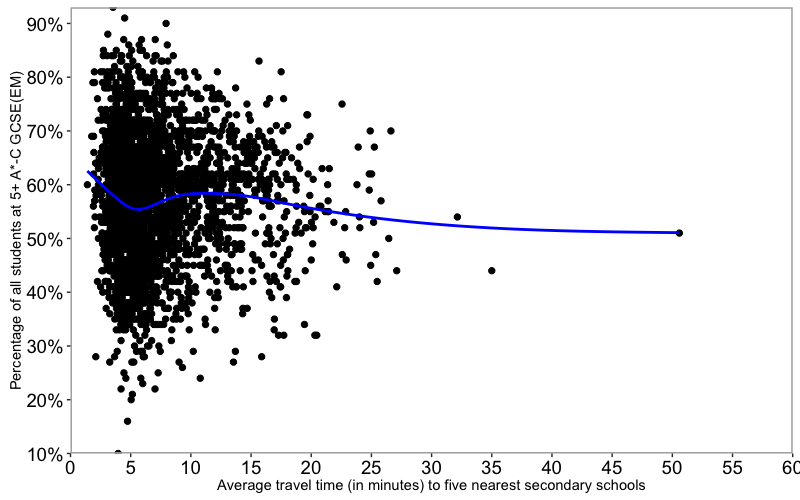
\includegraphics[width=\linewidth]{img/Figure1.jpg}
\end{figure}

\begin{figure}
\label{figure2}
\caption{Disadvantaged pupil attainment by Index of Isolation}
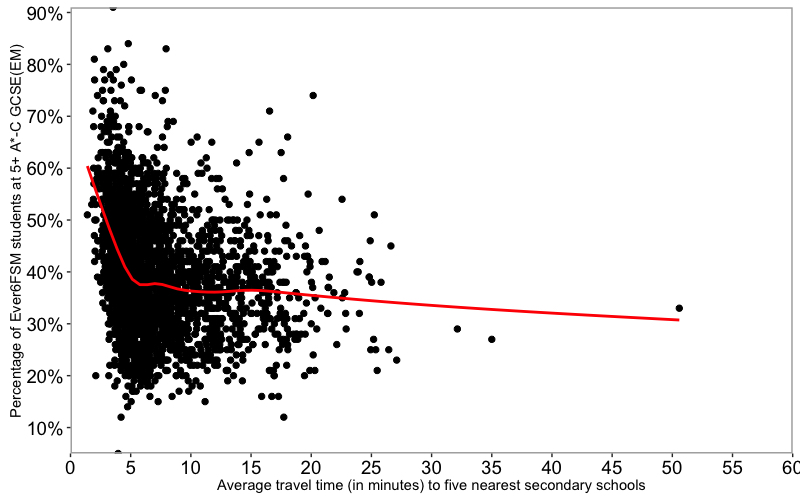
\includegraphics[width=\linewidth]{img/Figure2.jpg}
\end{figure}

\begin{table}[H]
	\centering
 \caption{Correlation between academic attainment and isolation, for all pupils and disadvantaged pupils} 
 \label{table1}
\begin{tabularx}{\linewidth}{|X|X|}
\hline
	All Pupils & Disadvantaged Pupils \\ 
	 \hline
 	-0.00085 & -0.22963 \\
 	\hline
 \end{tabularx}
\end{table}

% Table created by stargazer v.5.2 by Marek Hlavac, Harvard University. E-mail: hlavac at fas.harvard.edu
% Date and time: Mon, May 29, 2017 -- 16:51:38
\begin{sidewaystable}[!htbp] 
\centering 
 \caption{Academic Attainment by All Pupils and Disadvantaged Pupils, 2013--2015} 
 \label{table2} 
\begin{tabular}{@{\extracolsep{5pt}}lcccccc} 
\hline 
 & \multicolumn{6}{c}{\textit{Dependent variable:}} \\ 
\cline{2-7} 
\\[-1.8ex] & All Pupils & Disadvantaged Pupils & All Pupils & Disadvantaged Pupils & All Pupils & Disadvantaged Pupils\\ 
\\[-1.8ex] & (1) & (2) & (3) & (4) & (5) & (6)\\ 
\hline \\[-1.8ex] 
 IsoIndex & -0.0001 & -0.002$^{***}$ & -0.002$^{***}$ & -0.004$^{***}$ & -0.086$^{***}$ & -0.120$^{***}$ \\ 
  (0.0005) & (0.001) & (0.0004) & (0.0004)& (0.013) & (0.016) \\ 
 Ever6FSM & -0.246$^{***}$ & 0.082$^{***}$ & -0.265$^{***}$ & 0.010 & -0.266$^{***}$ & 0.039 \\
  (0.026) & (0.025) & (0.026) & (0.028) & (0.026) & (0.030) \\ 
 EAL & 0.161$^{***}$ & 0.208$^{***}$ & 0.126$^{***}$ & 0.156$^{***}$ & 0.157$^{***}$ & 0.166$^{***}$ \\ 
 & (0.016) & (0.014) & (0.014) & (0.016) & (0.018) & (0.020) \\ 
 SEN & -0.016 & 0.082 & 0.115 & 0.182 & 0.014 & 0.019 \\ 
 & (0.131) & (0.132) & (0.124) & (0.133) & (0.015) & (0.017) \\ 
 GIRLS & 0.076$^{***}$ & 0.065$^{***}$ & 0.077$^{***}$ & 0.074$^{***}$ & 0.095$^{***}$ & 0.105$^{***}$ \\
 & (0.012) & (0.012) & (0.012) & (0.013) & (0.015) & (0.018) \\ 
 TotPups & 0.00004$^{***}$ & 0.00002$^{***}$ & 0.00005$^{***}$ & 0.00003$^{***}$ & 0.146$^{***}$ & 0.127$^{***}$ \\ 
 & (0.00000) & (0.00001) & (0.00000) & (0.00001) & (0.015) & (0.017) \\ 
 KS2APS & 0.053$^{***}$ & 0.048$^{***}$ & 0.055$^{***}$ & 0.044$^{***}$ & 0.412$^{***}$ & 0.341$^{***}$ \\ 
 & (0.003) & (0.003) & (0.003) & (0.003) & (0.021) & (0.024) \\ 
 IDACI & -0.130$^{***}$ & -0.013 & -0.132$^{***}$ & -0.039$^{*}$ & -0.138$^{***}$ & -0.024 \\ 
 & (0.016) & (0.016) & (0.015) & (0.017) & (0.016) & (0.018) \\ 
 London & 0.062$^{***}$ & 0.091$^{***}$ & 0.074$^{***}$ & 0.102$^{***}$ & 0.615$^{***}$ & 0.978$^{***}$ \\ 
 & (0.006) & (0.006) & (0.005) & (0.006) & (0.045) & (0.046) \\ 
 Constant & -0.923$^{***}$ & -1.039$^{***}$ & -0.938$^{***}$ & -0.885$^{***}$ & -0.110$^{***}$ & -0.151$^{***}$ \\ 
 & (0.082) & (0.081) & (0.081) & (0.087) & (0.015) & (0.017) \\ 
 \hline \\[-1.8ex] 
Observations & 2,577 & 2,577 & 2,577 & 2,577 & 2,577 & 2,577 \\ 
R$^{2}$ & 0.467 & 0.408 & 0.507 & 0.323 & 0.507 & 0.332 \\ 
Adjusted R$^{2}$ & 0.465 & 0.406 & 0.505 & 0.321 & 0.505 & 0.330 \\ 
Res. Std. Err. & 1.193 & 0.653 & 0.002 & 0.002 & 0.014 & 0.015 \\ 
 (df=2567) & & & & & &\\ 
F Statistic & 250.185$^{***}$ & 196.556$^{***}$ & 293.005$^{***}$ & 136.171$^{***}$ & 293.005$^{***}$ & 141.700$^{***}$ \\ 
(df=9; 2567) & & & & & &\\ 
\hline 
\textit{Note:} & \multicolumn{6}{r}{$^{*}$p$<$0.05; $^{**}$p$<$0.01; $^{***}$p$<$0.001} \\ 
\end{tabular}
\end{sidewaystable} 

\section{Discussion}

\subsection{All Pupils}

Models 1, 3 and 5 in Table 2 analyse the relationship between the index of isolation and whole-school attainment of 5+ A*-C GCSE(EM). There is no statistically significant relationship between isolation and attainment in Model 1, and the effect size is small, a reduction in the attainment rate of 0.1 percentage points for each additional minute of average driving time to the five nearest schools. When the Index of Isolation is treated as a continuous treatment, as in Model 3, the effect size doubles, and there is a statistically significant negative relationship between isolation and attainment, controlling for all other covariables. Model 3 shows that for each additional minute in average travel time to the five nearest secondary schools, the proportion of pupils attaining 5+ A*-C GCSE(EM) decreases by 0.2 percentage points. In Model 5 the relationship between isolation and lower attainment is even clearer, with an increase of one standard deviation in travel time (equal to about 4.3 minutes of driving) is associated with a decline of 0.086 standard deviations in all pupil attainment, or one percentage point. Although the effect is smaller than all other independent variables it is nonetheless significant, and is strong evidence that, other school characteristics being equal, schools in more isolated areas have lower attainment rates.

\subsection{Disadvantaged Pupils}

As seen in Models 2, 4 and 6 in Table 2, the percentage of disadvantaged pupils in a school attaining 5+ A*-C GCSE(EM) Key Stage 4 is lower in more isolated schools, even when controlling for school demographics, previous pupil attainment, the local index of deprivation and whether the school is in London. This provides stronger evidence than previously available that disadvantaged pupils in less-populated areas of England have lower attainment than their disadvantaged peers in more urban and densely populated regions.

The effect of increased isolation on the academic attainment of disadvantaged pupils is small, with a decrease in the proportion of disadvantaged pupils in a school attaining 5+A*-C GCSE(EM) of 0.2 percentage points for each additional minute in average driving time to the five nearest secondary schools, as shown in Model 2. This increases to 0.4 percent for each additional minute when treating isolation as a continuous treatment variable uncorrelated with the other independent variables, as in Model 4. The relationship between isolation and lower disadvantaged pupil attainment is also clear in Model 6, with an increase of one standard deviation in travel time associated with a decline of 0.12 standard deviations in disadvantaged pupil attainment, equal to a 1.4 percentage point decline in the proportion of disadvantaged pupils achieving 5+A*-C GCSE(EM). This is a much larger effect size than seen in all-pupil attainment, and has a larger effect on disadvantaged pupil attainment than the proportion of girls, disadvantaged pupils, SEN pupils and the school's local IDACI score. In practice this is likely to mean only a small decrease, or no change at all, in the number of disadvantaged pupils achieving the 5+A*-C GCSE(EM) standard in a single school, given the three year average of 51.13 disadvantaged pupils per cohort, but across all schools it raises the possibility of hundreds of disadvantaged pupils each year who would have achieved the 5+A*-C GCSE(EM) standard in a less isolated school, but who do not because of their school's isolation.

There is not a gradual decline in disadvantaged pupil attainment the more isolated the school is, but a sharp drop in attainment once schools start to become more isolated from each other. This is illustrated in Figure 2, where disadvantage attainment in the least isolated schools is around 60\%, but drops to under 40\% in schools with an average travel time of just five minutes to their five nearest schools. A relatively small increase in isolation is correlated with disadvantaged attainment rates dropping by a third. This suggests the geographic divide between schools with higher and lower disadvantaged pupil attainment is not a divide between rural and urban areas, but between urban and suburban areas, or larger and smaller urban centres.

\subsection{Limitations and Suggestions for Future Research}

This analysis used only school level data, not individual pupil data, and so it does not include some demographic variables that may influence academic attainment. It is well documented that white pupils and black pupils have lower academic attainment than pupils of other ethnic backgrounds when not controlling for disadvantage \autocites{departmentforeducation2014b, departmentforeducation2015b, departmentforeducation2016}. Information on the ethnic makeup of individual school populations is not included in the DfE performance table data used in this analysis, and so I was unable to account for the ethnic background of each school's pupils. Urban areas also tend to have a greater proportion of non-white pupils than rural areas \autocites{officefornationalstatistics2013}, so the findings in this paper could be partially or entirely due to those ethnic demographic variables not included in the model.

It must be borne in mind that further research is needed to identify whether there is any causal link between the geographic isolation of a school and the academic attainment of disadvantaged pupils in that school. Research with pupil level data would allow for other variables, such as pupils' travel times to their nearest schools, ethnicity and other background characteristics, to be included in the analysis. While I have identified higher disadvantaged pupil attainment rates in less isolated schools, the data used does not allow for differentiating between different factors that could influence attainment, including the schools themselves, the effect of competition or collaboration between schools and background characteristics of the pupils attending those schools.

\section{Conclusion}

The relationship between increased levels of school isolation and lower academic attainment rate is worrying, particularly for disadvantaged pupils, due to their much lower attainment rate overall. While the aim of education policy is to provide all children in a society with fair and equitable access to the benefits of an education, it appears that pupils at schools in the more remote areas of England, particularly disadvantaged pupils, are not enjoying the same access to education and opportunities for achievement as their peers in areas of denser population. Furthermore, when framing the challenges of providing equitable opportunities and education, broader contexts beyond pupil characteristics, such as geographic isolation, must be taken into consideration.

While both competition and collaboration between schools may have contributed to rising pupil attainment in England, it seems that disadvantaged pupils in more isolated areas lag behind their more urban peers. These findings suggest that disadvantaged pupils in less densely populated areas of England are particularly under-serviced and under-supported. They have limited choices between schools, and those schools have limited options for collaboration. There may be additional challenges and barriers to disadvantaged pupil attainment in rural areas that have not been identified in the literature, in addition to those previously discussed. Future educational improvement policies and initiatives should, therefore, ensure that pupils in less populated areas -- particularly disadvantaged pupils -- have access to the same resources and opportunities as their peers in more populous and school-dense regions of the country.

\section*{Acknowledgements}

Thank you to Katy Theobald at The Future Leaders Trust for her comments on an earlier draft of this paper and to Meenakshi Parameshwaran at the Education Datalab for her advice and support on statistical methods.


\printbibliography

\end{document}
